\documentclass{beamer}
\mode<presentation>
\usepackage{amsmath,amssymb,mathtools}
\usepackage{textcomp}
\usepackage{gensymb}
\usepackage{adjustbox}
\usepackage{subcaption}
\usepackage{enumitem}
\usepackage{multicol}
\usepackage{listings}
\usepackage{url}
\usepackage{graphicx} % <-- needed for images
\def\UrlBreaks{\do\/\do-}

\usetheme{Boadilla}
\usecolortheme{lily}
\setbeamertemplate{footline}{
  \leavevmode%
  \hbox{%
  \begin{beamercolorbox}[wd=\paperwidth,ht=2ex,dp=1ex,right]{author in head/foot}%
    \insertframenumber{} / \inserttotalframenumber\hspace*{2ex}
  \end{beamercolorbox}}%
  \vskip0pt%
}
\setbeamertemplate{navigation symbols}{}

\lstset{
  frame=single,
  breaklines=true,
  columns=fullflexible,
  basicstyle=\ttfamily\tiny   % tiny font so code fits
}

\numberwithin{equation}{section}

% ---- your macros ----
\providecommand{\nCr}[2]{\,^{#1}C_{#2}}
\providecommand{\nPr}[2]{\,^{#1}P_{#2}}
\providecommand{\mbf}{\mathbf}
\providecommand{\pr}[1]{\ensuremath{\Pr\left(#1\right)}}
\providecommand{\qfunc}[1]{\ensuremath{Q\left(#1\right)}}
\providecommand{\sbrak}[1]{\ensuremath{{}\left[#1\right]}}
\providecommand{\lsbrak}[1]{\ensuremath{{}\left[#1\right.}}
\providecommand{\rsbrak}[1]{\ensuremath{\left.#1\right]}}
\providecommand{\brak}[1]{\ensuremath{\left(#1\right)}}
\providecommand{\lbrak}[1]{\ensuremath{\left(#1\right.}}
\providecommand{\rbrak}[1]{\ensuremath{\left.#1\right)}}
\providecommand{\cbrak}[1]{\ensuremath{\left\{#1\right\}}}
\providecommand{\lcbrak}[1]{\ensuremath{\left\{#1\right.}}
\providecommand{\rcbrak}[1]{\ensuremath{\left.#1\right\}}}
\theoremstyle{remark}
\newtheorem{rem}{Remark}
\newcommand{\sgn}{\mathop{\mathrm{sgn}}}
\providecommand{\abs}[1]{\left\vert#1\right\vert}
\providecommand{\res}[1]{\Res\displaylimits_{#1}}
\providecommand{\norm}[1]{\lVert#1\rVert}
\providecommand{\mtx}[1]{\mathbf{#1}}
\providecommand{\mean}[1]{E\left[ #1 \right]}
\providecommand{\fourier}{\overset{\mathcal{F}}{ \rightleftharpoons}}
\providecommand{\system}{\overset{\mathcal{H}}{ \longleftrightarrow}}
\providecommand{\dec}[2]{\ensuremath{\overset{#1}{\underset{#2}{\gtrless}}}}
\newcommand{\myvec}[1]{\ensuremath{\begin{pmatrix}#1\end{pmatrix}}}
\let\vec\mathbf

\title{Matgeo Presentation - Problem 12.76}
\author{ee25btech11063 - Vejith}

\begin{document}


\frame{\titlepage}
\begin{frame}{Question}
Four points  $\Vec{P}$ \brak{0,1}, $\Vec{Q}$ \brak{0,-3}, $\Vec{R}$ \brak{-2,-1}, $\Vec{S}$ \brak{2,-1} represent the vertices of a quadrilateral. What is  the area enclosed by the quadrilateral ?
\hfill (ST 2022)

(a) 4 \\
(b) 4$\sqrt{2}$ \\
(c) 8 \\
(d) 8$\sqrt{2}$

\end{frame}

\begin{frame}{Solution}
    \begin{align}
\vec{P} = \myvec{0 \\ 1} \hspace{0.8cm}
\vec{Q} = \myvec{0 \\ -3} \hspace{0.8cm}
\vec{R} = \myvec{-2 \\ -1} \hspace{0.8cm}
\vec{S} = \myvec{2 \\ -1}
\end{align}
let PSQR be the quadrilateral then it's diagonals are $\vec{P}-\vec{Q}$ and $\vec{R}-\vec{S}$\\
\begin{align}
    \norm{\vec{P}-\vec{Q}}=\norm{\myvec{0\\4}}=4\\
    \norm{\vec{R}-\vec{S}}=\norm{\myvec{-4\\0}}=4\\
    \brak{\vec{P}-\vec{Q}}^{\top}\brak{\vec{R}-\vec{S}}=\brak{0\hspace{0.5cm} 4}\myvec{-4\\0}\\
    =0
    \end{align}
    $\implies$ diagonals of the quadrilateral are of equal length and they bisect each other perpendicularly \\
     $\implies$ the given quadrilateral is a square
\end{frame}

\begin{frame}{Conclusion}
     \begin{align}
         \text{area of the quadrilateral PSQR}=\frac{1}{2} \norm{\vec{P}-\vec{Q}}^2\\
         =\frac{1}{2}\times 16 =8
     \end{align}
\end{frame}

\begin{frame}{Plot}
    \begin{figure}
    \centering
    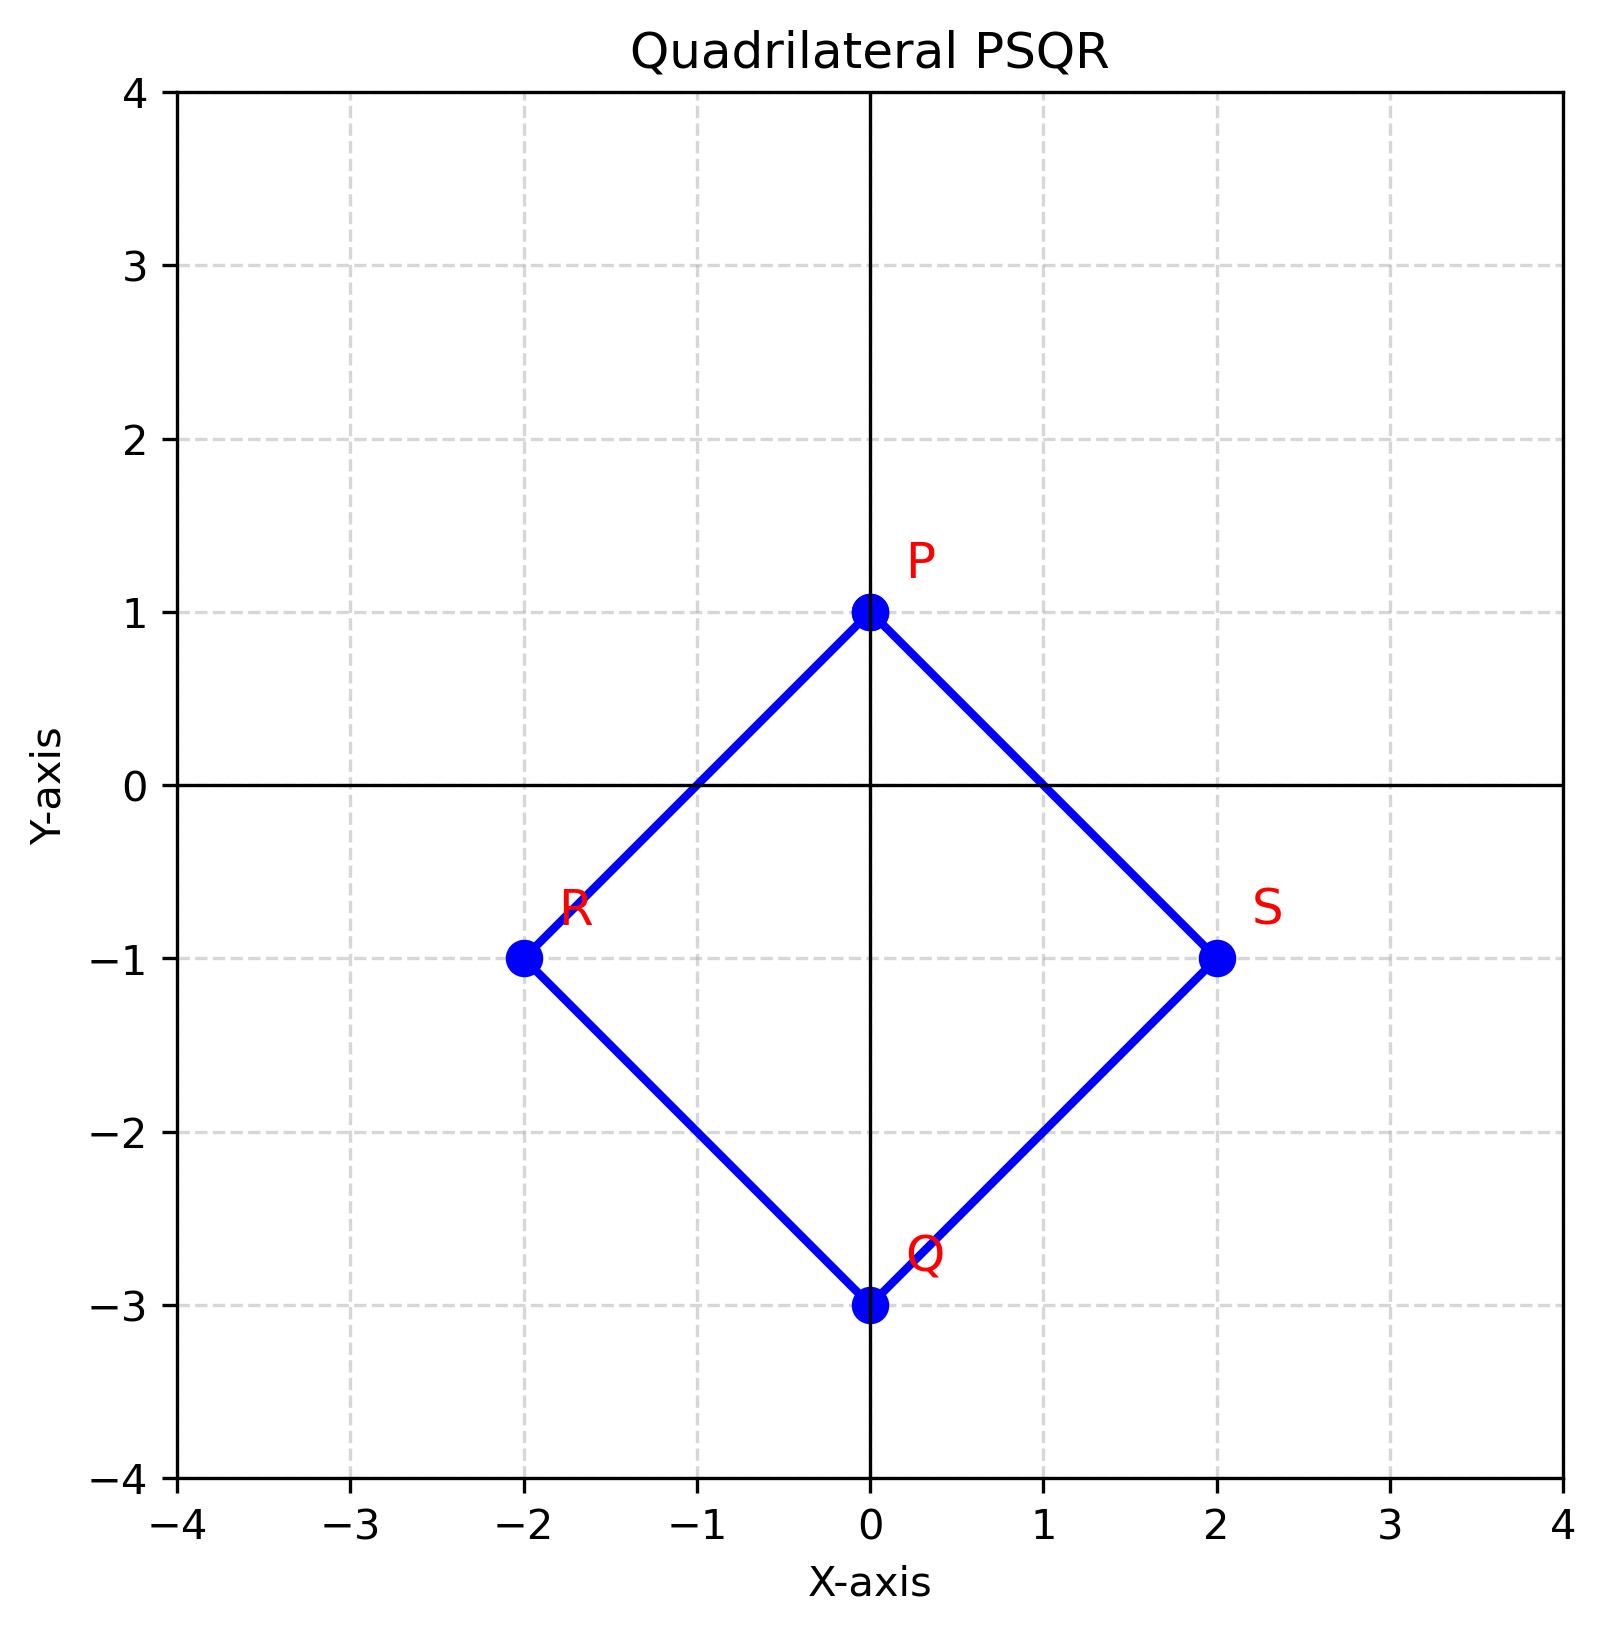
\includegraphics[width=0.6\columnwidth]{figs/01.png}
    \caption{}
    \label{fig:placeholder}
\end{figure}
\end{frame}

% --------- CODE APPENDIX ---------
\section*{Appendix: Code}

% C program
\begin{frame}[fragile]{C Code: area.c}
\begin{lstlisting}[language=C]
#include <stdio.h>
#include <math.h>

int main() {
    // Coordinates
    float x[4] = {0, 0, -2, 2};
    float y[4] = {1, -3, -1, -1};
    float area;
    float sum1 = 0, sum2 = 0;

    // Shoelace formula: sum over vertices
    for(int i = 0; i < 4; i++) {
        int j = (i + 1) % 4;
        sum1 += x[i] * y[j];
        sum2 += y[i] * x[j];
    }
    area = fabs(sum1 - sum2) / 2.0;

    // Calculate side lengths
    float pq = sqrt(pow(x[1]-x[0],2) + pow(y[1]-y[0],2));
    float qr = sqrt(pow(x[2]-x[1],2) + pow(y[2]-y[1],2));
    float rs = sqrt(pow(x[3]-x[2],2) + pow(y[3]-y[2],2));
    float sp = sqrt(pow(x[0]-x[3],2) + pow(y[0]-y[3],2));

    // Check type
    char type[20];
    if (fabs(pq - qr) < 1e-3 && fabs(qr - rs) < 1e-3 && fabs(rs - sp) < 1e-3)
        sprintf(type, "Square");
    else if (fabs(pq - rs) < 1e-3 && fabs(qr - sp) < 1e-3)
        sprintf(type, "Rectangle");
    else
        sprintf(type, "Other Quadrilateral");
\end{lstlisting}
\end{frame}

\begin{frame}[fragile]{C Code: area.c}
\begin{lstlisting}[language=C]
    // Write to file
    FILE *fp = fopen("area.dat", "w");
    if (fp == NULL) {
        printf("Error opening file!\n");
        return 1;
    }

    fprintf(fp, "Area of the quadrilateral = %.2f\n", area);
    fprintf(fp, "Type of quadrilateral = %s\n", type);

    fclose(fp);

    printf("Output written to area.dat successfully.\n");
    return 0;
}
\end{lstlisting}
\end{frame}

% Python plotting
\begin{frame}[fragile]{Python: plot.py}
\begin{lstlisting}[language=Python]
import numpy as np
import matplotlib.pyplot as plt

# Points
P = (0, 1)
Q = (0, -3)
R = (-2, -1)
S = (2, -1)

# Order: P → S → Q → R → P
x = [P[0], S[0], Q[0], R[0], P[0]]
y = [P[1], S[1], Q[1], R[1], P[1]]

# Plot
plt.figure(figsize=(6,6))
plt.plot(x, y, 'b-o', linewidth=2, markersize=8)
points = {'P': P, 'Q': Q, 'R': R, 'S': S}
for name, (x_pt, y_pt) in points.items():
    plt.text(x_pt + 0.2, y_pt + 0.2, name, fontsize=12, color='red')
limit = 4  
plt.xlim(-limit, limit)
plt.ylim(-limit, limit)
plt.gca().set_aspect('equal', adjustable='box')  # equal scaling

# Axes & grid
plt.axhline(0, color='black', linewidth=0.8)
plt.axvline(0, color='black', linewidth=0.8)
plt.grid(True, linestyle='--', alpha=0.5)
plt.xlabel("X-axis")
plt.ylabel("Y-axis")
plt.title("Quadrilateral PSQR")
plt.savefig("plot.png", dpi=300, bbox_inches='tight')
plt.show()
\end{lstlisting}
\end{frame}
\end{document}
